
\section{A prototype of an optimisation method}

Most, if not all, optimisation methods are based on the conceptual notion of successively obtaining \emph{directions} of potential improvement and suitable \emph{step sizes} in this direction, until a convergence or termination criterion (collectively called stopping criteria) is satisfied.

Considering what we have seen so far, we have now the concepts required for describing several unconstrained optimisation methods. We start by posing a conceptual optimisation algorithm in a pseudocode structure. This will be helpful in identifying the elements that differentiate the methods we will discuss.

%\captionsetup[algorithm]{font=footnotesize} 
\begin{algorithm}[H]
\caption{Conceptual optimisation algorithm} \label{Alg1}
\begin{algorithmic}[1] %line numbering frequency.
\State {\bf initialise.} iteration count $k = 0$, starting point $x_0$ 
\While {stopping criteria are not met} 
\State compute direction $d_k$ 
\State compute step size $\lambda_k $ %> 0$ 
\State $x_{k+1} = x_k + \lambda_k d_k$
\State $k = k+1$
\EndWhile
\State {\bf return} $x_k$.
\end{algorithmic}
\end{algorithm}

Algorithm \ref{Alg1} has two main elements, namely the computation of the direction $d_k$ and the step size $\lambda_k$ at each iteration $k$. In what follows, we present some univariate optimisation methods that can be employed to calculate step sizes $\lambda_k$. These methods are commonly referred to as \emph{line search methods}.

\section{Line search methods}

Finding an optimal step size $\lambda_k$ is in itself an optimisation problem. The name line search refers to the fact that it consists of a unidimensional search as $\lambda_k \in \reals$. 

Suppose that $f: \reals^n \mapsto \reals$ is differentiable. We define the unidimensional function $\theta: \reals \mapsto \reals$ as
%
\begin{align*}
\theta(\lambda) = f(x + \lambda d).
\end{align*}
%
Assuming differentiability, we can use the first-order necessary condition $\theta'(\lambda) = 0$ to obtain optimal values for the step size $\lambda$. This means solving the system
%
\begin{align*}
\theta'(\lambda) = d^\top\nabla f(x + \lambda d) = 0
\end{align*}
%
which might pose challenges. First, $d^\top\nabla f(x + \lambda d)$ is often nonlinear in $\lambda$, with optimal solutions not trivially resting at boundary points for an explicit domain of $\lambda$. Moreover, recall that $\theta'(\lambda) = 0$ is not a sufficient condition for optimality in general, unless  properties such as convexity can be inferred. 

In what follows, we assume that strict quasiconvexity holds and therefore $\theta'(\lambda) = 0$ becomes necessary and sufficient for optimality. In some contexts, unidimensional strictly quasiconvex functions are called \emph{unimodal}.

Theorem \ref{thm:line_search_red} establishes the mechanism underpinning line search methods. In that, we use the assumption that the function has a unique minimum (a consequence of being strictly quasiconvex) to successively reduce the search space until the optimal is contained in a sufficiently small interval $l$ within an acceptable tolerance.
%
\begin{theorem}[Line search reduction]\label{thm:line_search_red}
Let $\theta:\reals \rightarrow \reals$ be strictly quasiconvex over the interval $[a,b]$, and let $\lambda, \mu \in [a,b]$ such that $\lambda < \mu$. If $\theta(\lambda) > \theta(\mu)$, then $\theta(z) \geq \theta(\mu)$ for all $z \in [a,\lambda]$. If $\theta(\lambda) \leq \theta(\mu)$, then $\theta(z) \geq \theta(\lambda)$ for all $z \in [\mu, b]$.
\end{theorem}

\begin{figure}[H]
	\begin{tikzpicture}
%		\draw[help lines] (-5,-2) grid (5,2);
		\node (pic) at (0,0) {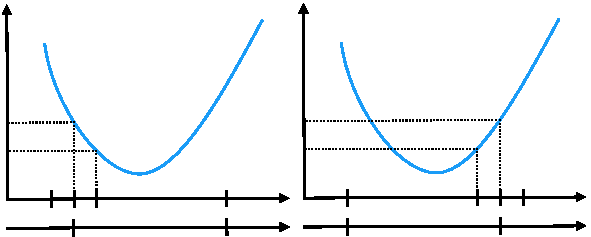
\includegraphics{part_2/chapter_5/figures/line_search.pdf}};
		\node (theta1) at (-1.15, 1.5) {$\theta$};
		\node (theta2) at (3.9, 1.5) {$\theta$};
		\node (theta_lambda1) at (-5.3, 0) {$\theta(\lambda)$};
		\node (theta_mu1) at (-5.3, -0.5) {$\theta(\mu)$};
		\node (a1) at (-4.15, -1) {$a$};
		\node (b1) at (-1.15, -1) {$b$};
		\node (lambda1) at (-3.75, -0.95) {$\lambda$};
		\node (mu1) at (-3.4, -1) {$\mu$};
		\node (a2) at (-3.75, -2.2) {$a$};
		\node (b2) at (-1.15, -2.2) {$b$};
		\node (theta_lambda2) at (-0.3, -0.5) {$\theta(\lambda)$};
		\node (theta_mu2) at (-0.3, 0) {$\theta(\mu)$};
		\node (lambda2) at (3.05, -0.95) {$\lambda$};
		\node (mu2) at (3.45, -1) {$\mu$};
		\node (a3) at (0.85, -1) {$a$};
		\node (b3) at (3.9, -1) {$b$};								
		\node (a4) at (0.85, -2.2) {$a$};
		\node (b4) at (3.5, -2.2) {$b$};					
	\end{tikzpicture}
	\caption{Applying Theorem \ref{thm:line_search_red} allows to iteratively reduce the search space.}\label{fig:line_search_reduction}
\end{figure}

Figure \ref{fig:line_search_reduction} provides an illustration of Theorem \ref{thm:line_search_red}. The line below the x-axis illustrates how the search space can be reduced between two successive iterations. In fact, most line search methods will iteratively reduce the search interval (represented by $[a,b]$) until the interval is sufficiently small to be considered ``a point'' (i.e., is smaller than a set threshold $l$).

Line searches are \emph{exact} when optimal step sizes $\lambda_k^*$ are calculated at each iteration $k$, and inexact when arbitrarily good approximations for $\lambda_k^*$ are used instead. As we will see, there is a trade-off between the number iterations required for convergence and the time taken per iteration that must be taken into account when choosing between exact and inexact line searches.

\subsection{Exact line searches}

Exact methods are designed to return the optimal step value $\lambda^*$ within a pre-specified tolerance $l$. In practice, it means that these methods return an interval $[a_k, b_k]$ such that $b_k - a_k \leq l$. 

\subsubsection{Uniform search}

The uniform search consists of breaking the search domain $[a,b]$ into N slices of uniform size $\delta = \frac{\lvert b-a \rvert}{N}$. This leads to a one-dimensional grid with grid points $a_n = a_0 + n\delta, n = 0 \dots N$ where $a_0 = a$ and $a_N = b$. We can then set $\hat{\lambda}$ to be
\begin{align*}
\hat{\lambda} = \arg\min_{i=0,\dots,n} f(a_i) 
\end{align*}

From Theorem \ref{thm:line_search_red}, we know that the optimal step size $\lambda^* \in [\hat{\lambda} -\delta, \hat{\lambda} + \delta]$. The process can then be repeated, by making $a = \hat{\lambda} -\delta$ and $b = \hat{\lambda} + \delta$ (see Figure \ref{fig:uniform_search}). until $|a - b|$ is less than a prespecified tolerance $l$. Without enough repetition of the search, the uniform search becomes an inexact search. 

This type of search is particularly useful when setting values for hyperparameters in algorithms (that is, user defined parameters that influence the behaviour of the algorithm) of performing any sort of search in a grid structure. One concept related to this type of search is what is known as the \emph{coarse-to-fine approach}. Coarse-to-fine approaches use sequences of increasingly fine approximations (i.e., gradually increasing $n$) to obtain computational savings in terms of function evaluations. In fact, the number of function evaluations a line search method executes is one of the indicators of its efficiency.
%
\begin{figure}[H]
	\centering
	\begin{tikzpicture}
%		\draw[help lines] (-3,-2) grid (3,2);
		\node (pic) at (0,0) {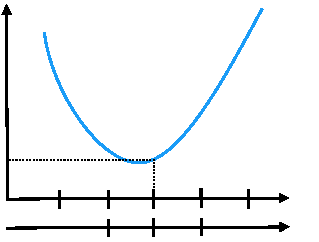
\includegraphics{part_2/chapter_5/figures/uniform.pdf}};
		\node (theta) at (1,1) {$\theta$};
		\node (a0) at (-1.95, -1.05) {$a=a_0$};
		\node (a1) at (-0.75, -1.05) {$a_1$};
		\node (a2) at (0.1, -1.05) {$a_2$};
		\node (a3) at (0.75, -1) {$\dots$};
		\node (b1) at (2, -0.95) {$a_n=b$};
		\node (lambdadelta1) at (-0.95, -2.25) {$\hat{\lambda} - \delta$};
		\node (lambdadelta2) at (0.75, -2.25) {$\hat{\lambda} + \delta$};
		\node (lambda) at (-0.1, -2.25) {$\hat{\lambda}$};
		\node (thetaa2) at (-3.1, -0.7) {$\theta(a_2)$};					
	\end{tikzpicture}
	\caption{Grid search with 5 points; Note that $\theta(a_2) = \min_{i=0,\dots,n} \theta(a_i)$.}	\label{fig:uniform_search}
\end{figure}
 
\subsubsection{Dichotomous search}

The \emph{dichotomous search} is an example of a sequential line search method, in which evaluations of the function $\theta$ at a current iteration $k$ are reused in the next iteration $k+1$ to minimise the number of function evaluations and thus improve performance. 

The word dichotomous refer to the mutually exclusive parts that the search interval $[a,b]$ is divided at each iteration. We start by defining a distance margin $\epsilon$ and defining two reference points $\lambda = \frac{a+b}{2} - \epsilon$ and $\mu = \frac{a+b}{2} + \epsilon$. Using the function values $\theta(\lambda)$ and $\theta(\mu)$, we proceed as follows.
%
\begin{enumerate}
\item If $\theta(\lambda) < \theta(\mu)$, then \emph{move to the left} by making $a_{k+1} = a_{k}$ and $b_{k+1} = \mu_k$;
\item Otherwise, if $\theta(\lambda) > \theta(\mu)$, then \emph{move to the right} by making $a_{k+1} = \lambda_{k}$ and $b_{k+1} = b_k$.
\end{enumerate}
%
Notice that, the assumption of strict quasiconvexity implies that $\theta(\lambda) = \theta(\mu)$ cannot occur, but in a more general setting one must make sure a criterion for resolving the tie. Once the new search interval $[a_{k+1}, b_{k+1}]$ is updated, new reference points $\lambda_{k+1}$ and $\mu_{k+1}$ are calculated and the process is repeated until $|a-b| \leq l$. The method is summarised in Algorithm \ref{Alg2}. Notice that, at any given iteration $k$, one can calculate what will be the size $|a_{k+1}-b_{k+1}|$, given by
%
\begin{align*}
b_{k+1} - a_{k+1} = \frac{1}{2^k}(b_0 - a_0) + 2\epsilon \left(1 - \frac{1}{2^k}\right ).
\end{align*}
%
This is useful in that it allows predicting the number of iterations Algorithm \ref{Alg2} will require before convergence. Figure \ref{fig:dichotomou_search} illustrates the process for two distinct functions. Notice that the employment of the central point $\frac{a+b}{2}$ as the reference to define the points $\lambda$ and $\mu$ turns the method robust in terms of interval reduction at each iteration.
%
\begin{algorithm}[H]
\caption{Dichotomous search} \label{Alg2}
\begin{algorithmic}[1] %line numbering frequency.
\State {\bf initialise.} distance margin $\epsilon > 0,$ tolerance $l > 0,$ $[a_0,b_0] = [a,b],$ $k = 0$ 
\While {$b_k - a_k > l$} 
\State $\lambda_k = \frac{a_k + b_k}{2} - \epsilon,$ $\mu_k = \frac{a_k + b_k}{2} + \epsilon$
\If {$\theta(\lambda_k) < \theta(\mu_k)$} \State $a_{k+1} = a_k,$ $b_{k+1} = \mu_{k}$
\Else \State $a_{k+1} = \lambda_k,$ $b_{k+1} = b_k$
\EndIf 
\State $k = k+1$
\EndWhile
\State {\bf return} $\overline{\lambda} = \frac{a_k + b_k}{2}$
\end{algorithmic}
\end{algorithm}
%
\begin{figure}[H]
	\begin{tikzpicture}
%		\draw[help lines] (-5,-2) grid (5,2);
		\node (pic) at (0,0) {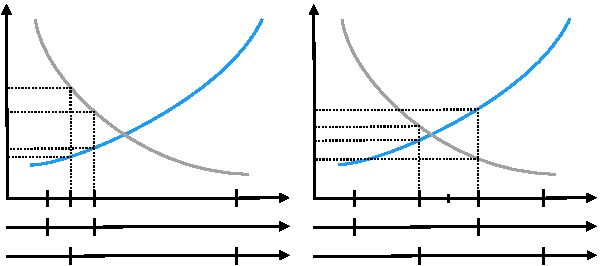
\includegraphics{part_2/chapter_5/figures/dichotomous.pdf}};
		\node (theta11) at (-1.3, 1.5) {$\theta_1$};
		\node (theta21) at (-1.15, -0.3) {$\theta_2$};
		\node (theta_mu1) at (-5.5, -0.1) {\small$\theta_1(\mu)$};
		\node (theta_lambda1) at (-5.5, -0.55) {\small$\theta_1(\lambda)$};
		\node (theta_mu2) at (-5.5, 0.4) {\small$\theta_2(\mu)$};
		\node (theta_lambda2) at (-5.5, 0.75) {\small$\theta_2(\lambda)$};
		\node (lambda_1) at (-3.9 ,-0.8) {$\lambda$};
		\node (mu_1) at (-3.5 ,-0.85) {$\mu$};
		\node (a1) at (-4.3, -0.8) {$a$};
		\node (a11) at (-4.3, -1.9) {$a$};
		\node (a21) at (-3.9, -2.4) {$a$};
		\node (b1) at (-1.1, -0.8) {$b$};
		\node (b11) at (-3.5, -1.9) {$b$};
		\node (b21) at (-1.1, -2.4) {$b$};
		%
		\node (theta21) at (4.15, -0.3) {$\theta_2$};
		\node (theta12) at (3.9, 1.5) {$\theta_1$};
		\node (theta_mu1) at (-0.25, 0.55) {\small$\theta_1(\mu)$};
		\node (theta_lambda1) at (-0.25, -0.2) {\small$\theta_1(\lambda)$};
		\node (theta_mu2) at (-0.25, -0.5) {\small$\theta_2(\mu)$};
		\node (theta_lambda2) at (-0.25, 0.2) {\small$\theta_2(\lambda)$};
		\node (lambda_2) at (2, -0.8) {$\lambda$};
		\node (mu_2) at (3 , -0.85) {$\mu$};
		\node (ab2) at (2.5 , -0.75) {\footnotesize$\frac{(a+b)}{2}$};
		\node (a1) at (0.9, -0.8) {$a$};
		\node (a11) at (0.9, -1.9) {$a$};
		\node (a21) at (2, -2.4) {$a$};
		\node (b1) at (4.1, -0.8) {$b$};
		\node (b11) at (3, -1.9) {$b$};
		\node (b21) at (4.1, -2.4) {$b$};													
	\end{tikzpicture}
	\caption{Using the midpoint $(a+b)/2$ and Theorem \ref{thm:line_search_red} to reduce the search space.} \label{fig:dichotomou_search}
\end{figure}

\subsubsection{Golden section search*}

The \emph{golden section search} is named after the \emph{golden ratio} $\varphi =  \frac{1 + \sqrt{5}}{2}$, of which the inverse is used as the ratio of reduction for the search interval $[a,b]$ at each iteration. 

Consider that, once again, we rely on two reference points $\lambda_k$ and $\mu_k$. The method is a consequence of imposing two requirements for the line search:
%
\begin{enumerate}
\item the reduction in the search interval should not depend on whether $\theta(\lambda_k) > \theta(\mu_k)$ or vice-versa.
\item at each iteration, we perform a single function evaluation, thus making $\lambda_{k+1} = \mu_{k}$ if $\theta(\lambda_k) > \theta(\mu_k)$ or vice-versa.
\end{enumerate}
% 
From requirement 1, we can infer that $b_{k+1} - a_{k+1} = b_k - \lambda_k = \mu_k - a_k$ is required. To find the interval reduction rate $\alpha \in (0,1)$ that would allow so, we define $\mu_k = a_k + \alpha(b_k - a_k)$ and, consequently, $\lambda_k = a_k + (1-\alpha)(b_k - a_k)$. Notice that this makes $b_{k+1} - a_{k+1} = \alpha(b_k - a_k)$.

Notice the following. Suppose that $\theta(\lambda_k) > \theta(\mu_k)$ at iteration $k$. We then make $a_{k+1} = \lambda_k$ and $b_{k+1} = b_k$, a "movement to the right". From requirement 2, we also make $\lambda_{k+1} = \mu_{k}$ so that $\theta(\lambda_{k+1}) = \theta(\mu_{k})$, avoiding a function evaluation. 

From the above, we can calculate the ratio $\alpha$ that would allow the method to work. Notice that
\begin{align*}
&\lambda_{k+1} = \mu_k \\
&a_{k+1} + (1-\alpha)(b_{k+1} - a_{k+1})  = \mu_k \\
&(1-\alpha)[\alpha(b_k - a_k)]  = \mu_k - \lambda_k \\
&(\alpha - \alpha^2)(b_k - a_k) = a_k+\alpha(b_k - a_k) - [a_k + (1-\alpha)(b_k - \alpha_k)] \\
&\alpha^2 + \alpha - 1 = 0
\end{align*}
to which $\alpha = \frac{2}{1 + \sqrt{5}} = 0.618... = \frac{1}{\varphi}$ is the positive solution. Clearly, the same result is obtained if one consider $\theta(\lambda_k) < \theta(\mu_k)$. Algorithm \ref{Alg3} summarises the golden section search. Notice that at each iteration, only a single additional function evaluation is required. 
%
\begin{algorithm}[H]
\caption{Golden section search} \label{Alg3}
\begin{algorithmic}[1] %line numbering frequency. 
\State {\bf initialise.} tolerance $l > 0,$ $[a_0,b_0] = [a,b],$ $\alpha = 0.618,$ $k = 0$ 
\State $\lambda_k = a_k + (1-\alpha)(b_k - a_k),$ $\mu_k = a_k + \alpha(b_k - a_k)$
\While {$b_k - a_k > l$} 
\If {$\theta(\lambda_k) > \theta(\mu_k)$} 
    \State $a_{k+1} = \lambda_k,$ $b_{k+1} = b_k,$ $\lambda_{k+1} = \mu_k,$ and
    \State $\mu_{k+1} = a_{k+1} + \alpha (b_{k+1} - a_{k+1})$. Calculate $\theta(\mu_{k+1})$
\Else 
    \State $a_{k+1} = a_k,$ $b_{k+1} = \mu_k,$ $\mu_{k+1} = \lambda_k,$ and
    \State $\lambda_{k+1} = a_{k+1} + (1-\alpha)(b_{k+1} - a_{k+1})$. Calculate $\theta(\lambda_{k+1})$
\EndIf 
\State $k \gets k+1$
\EndWhile
\State {\bf return} $\overline{\lambda} = \frac{a_k + b_k}{2}$
\end{algorithmic}
\end{algorithm}

Comparing the above method for a given accuracy $l$, the required number of function evaluations is:
$$\min \left\{ n : \begin{array}{l} \text{uniform: } n \geq \frac{b_1 - a_1}{l/2} - 1   \\
                               \text{dichotomous: } (1/2)^{n/2} \leq \frac{l}{b_1-a_1}  \\
                               \text{golden section: }(0.618)^{n-1} \leq \frac{l}{b_1-a_1} \\
                               %\text{Fibonacci section: }F_n \geq \frac{(b_1-a_1)}{l}                 
                               \end{array} \right\}
$$
For example: suppose we set $[a,b] = [-10,10]$ and $l = 10^{-6}$. Then the number of iterations required for convergence is 
%
\begin{itemize}
\item uniform: $n=4\times 10^6$; 
\item dichotomous: $n = 49$;  
\item golden section: $n=36$.
\end{itemize}
%
A variant of the golden section method uses Fibonacci numbers to define the ratio of interval reduction. Despite being marginally more efficient in terms of function evaluations, the overhead of calculating Fibonacci numbers has to be taken into account. 
 

\subsubsection{Bisection search}

Differently form the previous methods, the bisection search relies on derivative information to infer whether how the search interval should be reduced. For that, we assume that $\theta(\lambda)$ is differentiable and convex. 

We proceed as follows. If $\theta'(\lambda_k) = 0$, then $\lambda_k$ is a minimiser. Otherwise 
\begin{enumerate}
\item if $\theta'(\lambda_k) > 0$, then, for $\lambda > \lambda_k$, we have $\theta'(\lambda_k)(\lambda - \lambda_k) > 0$, which implies $\theta(\lambda) \geq \theta(\lambda_k)$ since $\theta$ is convex. Therefore, the new search interval becomes $[a_{k+1}, b_{k+1}] = [a_k,\lambda_k]$.
\item if $\theta'(\lambda_k) < 0$, we have $\theta'(\lambda_k)(\lambda - \lambda_k) > 0$ (and thus $\theta(\lambda) \geq \theta(\lambda_k)$) for $\lambda < \lambda_k$. Thus, the new search interval becomes $[a_{k+1}, b_{k+1}] = [\lambda_k, b_k]$.
\end{enumerate}
 
As in the dichotomous search, we set $\lambda_k = \frac{1}{2}(b_k + a_k)$, which provides robust guarantees of search interval reduction. Notice that the dichotomous search can be seen as a bisection search in which the derivative information is estimated using the difference of function evaluation at two distinct points. Algorithm \ref{Alg4} summarises the bisection method.

\begin{algorithm}[h]
\caption{Bisection method} \label{Alg4}
\begin{algorithmic}[1] %line numbering frequency.
\State {\bf initialise.} tolerance $l > 0,$ $[a_0,b_0] = [a,b],$ $k = 0$ 
\While {$b_k - a_k > l$} 
    \State $\lambda_k = \frac{(b_k + a_k)}{2}$ and evaluate $\theta'(\lambda_k)$
    \If {$\theta'(\lambda_k) = 0$} return $\lambda_k$
    \ElsIf {$\theta'(\lambda_k) > 0$} 
        \State $a_{k+1} = a_k,$ $b_{k+1} = \lambda_k$
    \Else
        \State $a_{k+1} = \lambda_k,$ $b_{k+1} = b_k$   
    \EndIf 
\State $k \gets k+1$
\EndWhile
\State {\bf return} $\overline{\lambda} = \frac{a_k + b_k}{2}$
\end{algorithmic}
\end{algorithm}


\subsection{Inexact line search}

Often, it is worth sacrificing optimality of the step size $\lambda^k$ for the overall efficiency of the solution method in terms of solution time. 

There are several heuristics that can be employed to define step sizes and their performance are related to how the directions $d_k$ are defined in Algorithm \ref{Alg1}. Next, we present the \emph{Armijo rule}, arguably the most used technique to obtain step sizes in efficient implementations of optimisation methods. 

\subsubsection{Armijo rule}

The Armijo rule is a condition that is tested to decide whether a current step size $\overline{\lambda}$ is acceptable or not. The step size $\overline{\lambda}$ is considered acceptable if
%
\begin{align*}
f(x + d\overline{\lambda}) - f(x) \leq \alpha \overline{\lambda}\nabla f(x)^\top d.
\end{align*}
%
One way of understanding the Armijo rule is to look at what it means in terms of the function $\theta(\lambda) = f(x +\lambda d)$. Notice that, at $\lambda = 0$, the Armijo rule becomes
\begin{align}
& \theta(\overline{\lambda}) - \theta(0) \leq \alpha \overline{\lambda} \theta'(0) \nonumber \\ 
& \theta(\overline{\lambda}) \leq \theta(0) + \alpha \overline{\lambda}\theta'(0) \label{eq:armijo_test}.
\end{align}
That is, $\theta(\overline{\lambda})$ has to be less than the deflected linear extrapolation of $\theta$ at $\lambda = 0$. The deflection is given by the pre-specified parameter $\alpha$. In case $\overline{\lambda}$ does not satisfy the test in \eqref{eq:armijo_test}, $\overline{\lambda}$ is reduced by a factor $\beta \in (0,1)$ until the test in \eqref{eq:armijo_test} is satisfied. 
%
\begin{figure}[H]
	\begin{tikzpicture}
%		\draw[help lines] (-5,-2) grid (5,2);
		\node (pic) at (0,0) {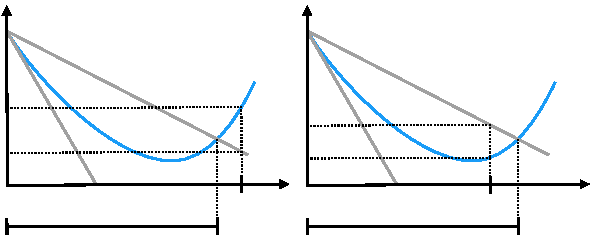
\includegraphics{part_2/chapter_5/figures/armijo.pdf}};
		\node (lambda) at (-0.9, -1.55) {$\overline{\lambda}$};
		\node (beta_lambda) at (3.2, -1.55) {$\beta\overline{\lambda}$};
		\node (acceptable1) at (-3, -2.1) {\footnotesize acceptable $\lambda_k$};
		\node (acceptable1) at (2, -2.1) {\footnotesize acceptable $\lambda_k$};
		\node (image_lin1) at (-5.35, -0.55) {\scriptsize$\theta_{\text{app}}(\overline{\lambda})$};
		\node (theta_lambda1) at (-5.2, 0.2) {\scriptsize$\theta(\overline{\lambda})$};
		\node (image_lin2) at (-0.35, -0.1) {\scriptsize$\theta_{\text{app}}(\overline{\beta\lambda})$};
		\node (theta_lambda2) at (-0.2, -0.7) {\scriptsize$\theta(\beta\overline{\lambda})$};
		\node (approx1)[right] at (-4.6, 1.5) {\footnotesize$\theta_{\text{app}}(\overline{\lambda})=\theta(0)+\alpha\overline{\lambda}(\theta'(0))$};
		\node (approx2)[right] at (0.5, 1.5) {\footnotesize$\theta_{\text{app}}(\overline{\lambda})=\theta(0)+\alpha\overline{\lambda}(\theta'(0))$};
		\node (lin1)[right] at (-4.5, -1.35) {\scriptsize$\theta(0)+\overline{\lambda}(\theta'(0))$};
		\node (lin2)[right] at (0.5, -1.35) {\scriptsize$\theta(0)+\overline{\lambda}(\theta'(0))$};
	\end{tikzpicture}
	\caption{At first $\lambda_0 = \overline{\lambda}$ is not acceptable; after reducing the step size to $\lambda_1 = \beta \overline{\lambda}$, it enters the acceptable range where $\theta(\lambda_k) \le \theta_{\text{app}}(\lambda_k)=\theta(0)+\alpha\lambda_k(\theta'(0))$.} \label{fig:armijo_rule}
\end{figure}

%
In Figure \ref{fig:armijo_rule}, we can see the acceptable region for the Armijo test. At first, $\overline{\lambda}$ does not satisfy the condition \eqref{eq:armijo_test}, being then reduced to $\beta\overline{\lambda}$, which, in turn, satisfies \eqref{eq:armijo_test}. In this case, $\lambda_k$ would have been set $\beta\overline{\lambda}$. Suitable values for $\alpha$ are within $(0,0.5]$ and for $\beta$ are within $(0,1)$, trading of precision (higher values) and number of tests before acceptance (lower values).

The Armijo rule is called \emph{backtracking} in some contexts, due to the successive reduction of the step size caused by the factor $\beta \in (0,1)$. Some variants might also include rules that prevent the step size from becoming too small, such as $\theta(\delta\overline{\lambda}) \geq \theta(0) + \alpha \delta\overline{\lambda}\theta'(0)$, with $\delta > 1$.
    
\section{Unconstrained optimisation methods}

We now focus on developing methods that can be employed to optimise $f: \reals^n \mapsto \reals$. We start with coordinate descent method, which is derivative free, to then discuss the gradient method and Newton's method. In essence, the main difference between the three methods is how the directions $d_k$ in Algorithm \ref{Alg1} are determined. Also, all of these methods rely on line searches to define optimal step sizes, which can be any of the methods seen before or any other unidimensional optimisation method.

\subsection{Coordinate descent}

The \emph{cordinate descent method} relies on a simple yet powerful idea. By focusing on one coordinate at the time, the method trivially derives directions $d$ having $d_i = 1$ for coordinate $i$ and $d_{j \neq i} = 0$ otherwise. As one would suspect, the order in which the coordinates are selected influences the performance of the algorithm. Some known variants include:
%
\begin{enumerate}
\item {\bf Cyclic:} coordinates are considered in order $1,\dots,n$;
\item {\bf Double-sweep:} swap the coordinate order at each iteration;
\item {\bf Gauss-Southwell:} choose components with largest $\frac{\partial f(x)}{\partial x_i}$;
\item {\bf Stochastic:} coordinates are selected at random.
\end{enumerate}
  

Algorithm \ref{Alg5} summarises the general structure of the coordinate descent method. Notice that the for-loop starting in Line \ref{alg5:line3} uses the cyclic variant of the coordinate descent method. 

%% Juho: Nicer caption + spacing
\begin{algorithm}[H]
\caption{Coordinate descent method (cyclic)} \label{Alg5}
\begin{algorithmic}[1] %line numbering frequency. 
\State {\bf initialise.} tolerance $\epsilon > 0,$ initial point $x^0,$ iteration count $k = 0$ 
\While {$||x^{k+1} - x^{k}|| > \epsilon$} 
    \For {$j = 1,\dots n$} \label{alg5:line3}
        \State $d =\braces{d_i = 1, \text{ if } i=j; d_i = 0, \text{ if } i \neq j}$
        \State $\overline{\lambda}_j = \argmin_{\lambda \in \reals}\braces{f(x_j^k + \lambda d_j)}$
        \State $x^{k+1}_j = x^k_j + \overline{\lambda}_j  d_j$
    \EndFor
    \State $k = k+1$
\EndWhile
\State {\bf return} $x^k$
\end{algorithmic}
\end{algorithm}

Figure \ref{fig:coordinate_descent} shows the progress of the algorithm when applied to solve 
$$f(x)=e^{(-(x_1-3)/2)} + e^{((4x_2 + x_1)/10)} + e^{((-4x_2 + x_1)/10)}$$ using the golden section method as line search. 

\begin{figure}[H]
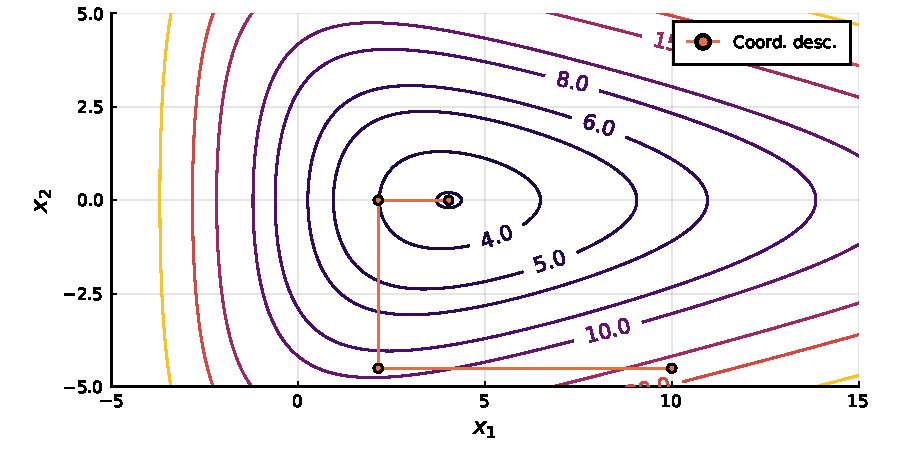
\includegraphics[width=0.8\textwidth]{part_2/chapter_5/figures/coordinate_decent_exact.pdf}	
\caption{Coordinate descent method applied to $f$. Convergence is observed in 4 steps for a tolerance $\epsilon = 10^{-5}$} \label{fig:coordinate_descent}
\end{figure}

The coordinate descent method is the strategy employed in several other methods, such as the \emph{Gauss-Seidel} method for solving linear system of equations, which is why some references refer to each of these iterations as Gauss-Seidel steps. Also, when a collection of coordinates is used to derive a direction, the term \emph{block coordinate descent} is used, though a method for deriving directions for each block is still necessary, for example the gradient method presented next.  


\subsection{Gradient (descent) method}

The \emph{gradient descent} uses the function gradients as the search direction $d$. Before we present the method, let us present a result that justifies the use of gradients to derive search directions. 

\begin{lemma}
Suppose that $f :\reals^n\hspace{-2pt} \rightarrow \reals$ is differentiable at $x\hspace{-1pt}\in\hspace{-1pt} \reals^n$ and $\nabla f(x) \neq 0$. Then $\overline{d} = -\frac{\nabla f(x)}{||\nabla f(x)||}$ is the direction of steepest descent of $f$ at $x$.
\end{lemma}
%
\begin{proof} From differentiability of $f$, we have
\begin{align*}
f'(x; d)& = \lim_{\lambda \rightarrow 0^+} \frac{f(x + \lambda d) - f(x)}{\lambda} = \nabla f(x)^\top d.	
\end{align*}
Thus, $\overline{d} = \argmin_{||d|| \leq 1}\braces{\nabla f(x)^\top d} = -\frac{\nabla f(x)}{||\nabla f(x)||}$
\end{proof}

In the proof, we use the differentiability to define a directional derivative for $f$ at direction $d$, that is, the change in the value of $f$ by a move of size $\lambda >0$ in the direction $d$, which is given by $\nabla f(x)^\top d$. If we minimise this term in $d$ for $||d||_2 \leq 1$, we observe that $d$ is a vector of length one that has the opposite direction of $\nabla f(x)$, thus $d = - \frac{\nabla f(\overline{x})}{||\nabla f(\overline{x})||}$. 

That provides us with the insight that we can use $\nabla f(\overline{x})$ to derive (potentially good) directions for optimising $f$. Notice that the direction employed is the opposite direction of the gradient for minimisation problems, being the opposite in case of maximisation. That is the reason why the gradient method is called the \emph{steepest descent} method in some references, though gradient and steepest descent might refer to different methods in specific contexts.

Using the gradient $\nabla f(\overline{x})$ is also a convenience as it allows for the definition of a straightforward convergence condition. Notice that, if $\nabla f(\overline{x}) = 0$, then the algorithm stalls, as $x_{k+1} = x_k + \lambda_k d_k = x_k$. In other words, the algorithm converges to points $x \in \reals^n$ that satisfy the first-order necessary conditions $\nabla f(\overline{x}) = 0$. 

The gradient method has many known variants that try to mitigate issues associated with the poor convergence caused by the natural 'zigzagging' behaviour of the algorithm (see, for example the gradient method \emph{with momentum} and the \emph{Nesterov} method). 

There are also variants that only consider the partial derivatives of some (and not all) of the dimensions $i = 1, \dots, n$ forming \emph{blocks} of coordinates at each iteration. If these blocks are randomly formed, these methods are known as \emph{stochastic gradient} methods. 

In Algorithm \ref{Alg6} we provide a pseudocode for the gradient method. In Line \ref{alg6:l2}, the stopping condition for the while-loop is equivalent of testing $\nabla f(\overline{x}) = 0$ for a tolerance $\epsilon$. 

\begin{algorithm}[H]
\caption{Gradient method} \label{Alg6}
\begin{algorithmic}[1] %line numbering frequency. 
\State {\bf initialise.} tolerance $\epsilon > 0,$ initial point $x_0,$ iteration count $k = 0$. 
\While {$||\nabla f(x_k)|| > \epsilon$} \label{alg6:l2}
        \State $d = -\frac{\nabla f(x_k)}{||\nabla f(\overline{x})||}$
        \State $\overline{\lambda} = \argmin_{\lambda \in \reals}\braces{f(x_k + \lambda d)}$
        \State $x_{k+1} = x_k + \overline{\lambda}  d_j$
    \State $k = k+1$    
\EndWhile
\State {\bf return} $x_k$.
\end{algorithmic}
\end{algorithm}

Figure \ref{fig:gradient} presents the progress of the gradient method using exact (bisection) and inexact (Armijo rule with $\alpha =0.1$ and $\beta=0.7$) line searches. As can be expected, when an inexact line search is employed, the method overshoots slightly some of the steps, taking a few more iterations to converge.  

\begin{figure}[h]
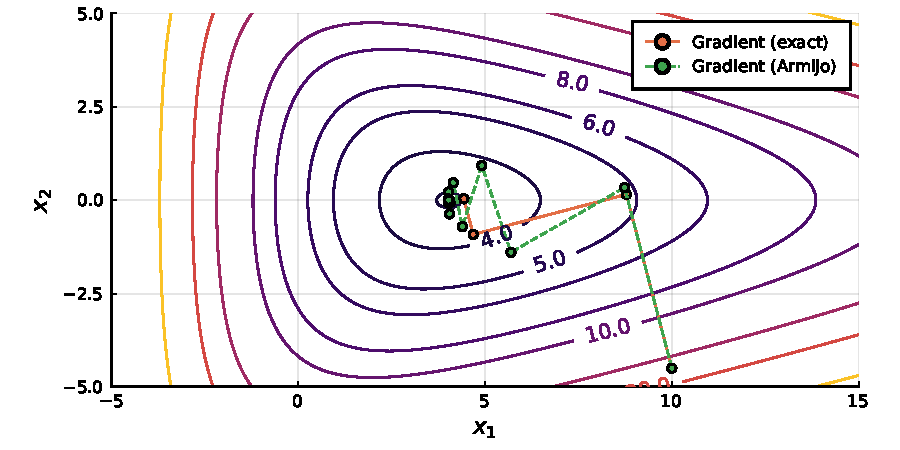
\includegraphics[width=0.9\textwidth]{part_2/chapter_5/figures/gradient.pdf}
\caption{Gradient method applied to $f$. Convergence is observed in 10 steps using exact line search and 19 using Armijo's rule (for $\epsilon = 10^{-5}$)} \label{fig:gradient}
\end{figure}


\subsection{Newton's method}

One can think of gradient methods as using first-order information to derive directions of improvement, while \emph{Newton's method} consists of a step forward also incorporating second-order information. This can be shown to produce better convergence properties, but at the expense of the extra computational burden incurred by calculating and manipulating Hessian matrices.

The idea of the Newton's method is the following. Consider the second-order approximation of $f$ at $x_k$, which is given by
%
\begin{align*}
q(x) = f(x_k) + \nabla f(x_k)^\top (x - x_k) + \frac{1}{2}(x - x_k)^\top H(x_k)(x - x_k)
\end{align*}
%

The method uses as direction $d$ that of the extremum of the quadratic approximation at $x_k$, which can be obtained from the first-order condition $\nabla q(x) = 0$. This renders
%
\begin{align}
\nabla q(x) = \nabla f(x_k) + H(x_k)(x - x_k) = 0. \label{eq:newton_cond}
\end{align}
%
Assuming that $H^{-1}(x_k)$ exists, we can use \eqref{eq:newton_cond} to obtain the following update rule, which is known as the \emph{Newton step}
%
\begin{align}
x_{k+1} = x_k - H^{-1}(x_k)\nabla f(x_k)	 \label{eq:newton_method}
\end{align}
%

Notice that the ``pure'' Newton's method has embedded in the direction of the step, its length (i.e., the step size) as well. In practice, the method uses $d = - H^{-1}(x_k)\nabla f(x_k)$ as a direction combined with a line search to obtain optimal step sizes and prevent divergence (that is, converge to $-\infty$) in cases where the second-order approximation might lead to divergence. Fixing $\lambda = 1$ renders the natural Newton's method, as derived in \eqref{eq:newton_method}. The Newton's method can also be seen as employing Newton-Raphson method to solve the system of equations that describe the first order conditions of the quadratic approximation at $x_k$. 

Figure \ref{fig:newton_method_exp} shows the calculation of direction $d = - H^{-1}(x_k)\nabla f(x_k)$ for the first iteration of the Newton's method. Notice that the direction is the same as the that of the minimum of the quadratic approximation $q(x)$ at $x_k$. The employment of a line search allows for overshooting the exact minimum, making the search more efficient.
%
\begin{figure}[H]
    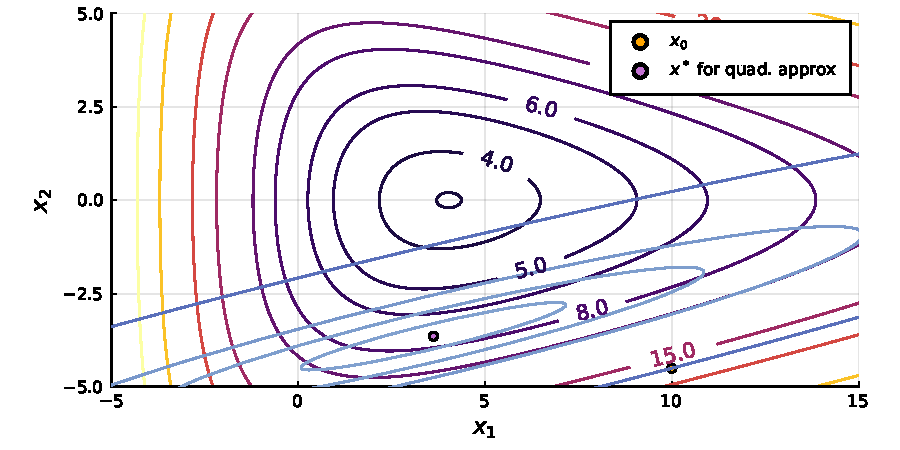
\includegraphics[width=0.49\textwidth]{part_2/chapter_5/figures/newton_path1.pdf}	
	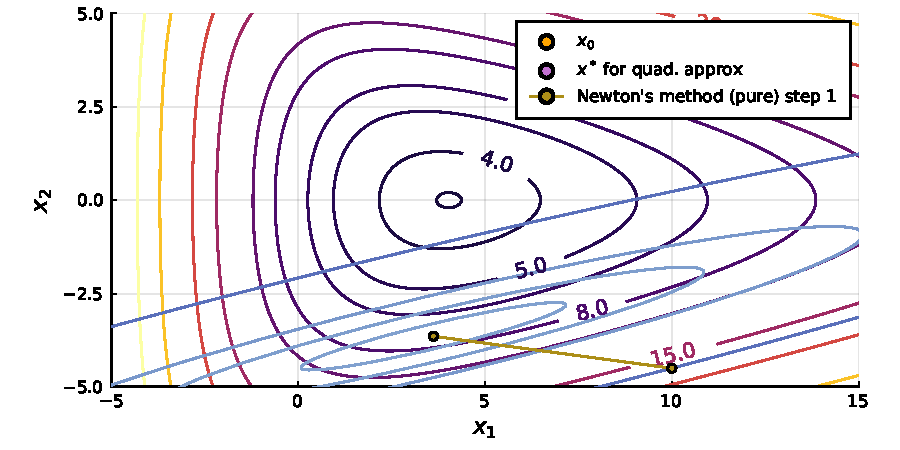
\includegraphics[width=0.49\textwidth]{part_2/chapter_5/figures/newton_path2.pdf}
	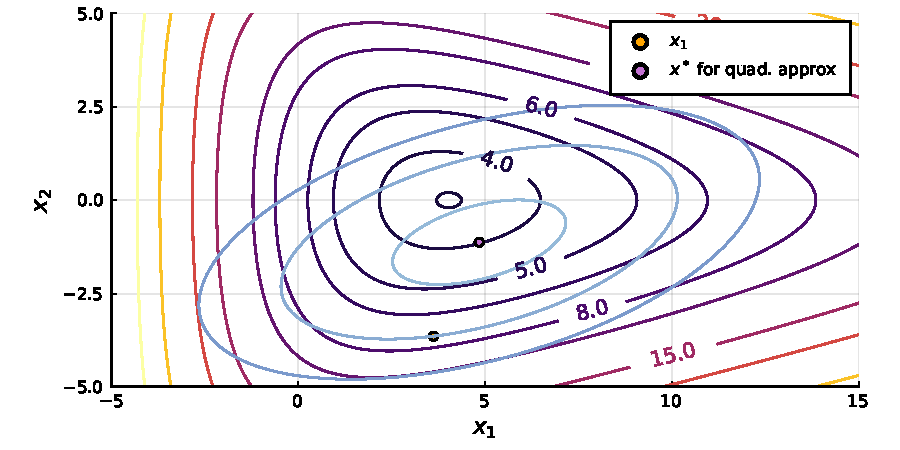
\includegraphics[width=0.49\textwidth]{part_2/chapter_5/figures/newton_path3.pdf}
	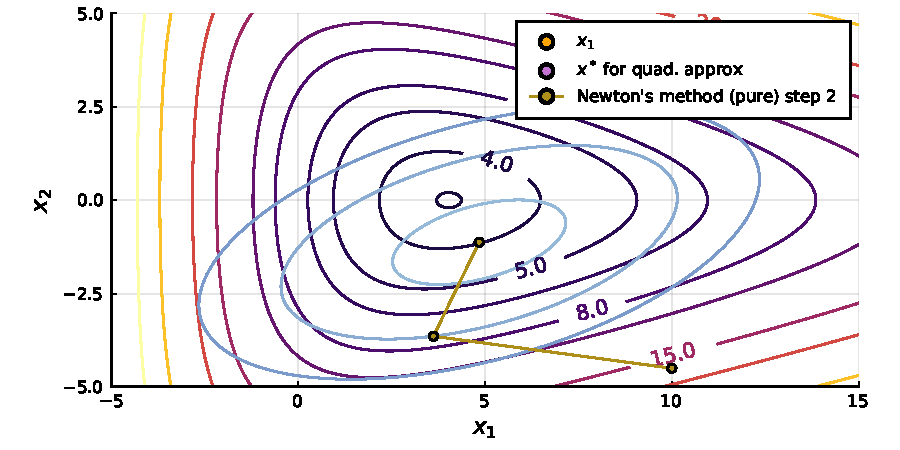
\includegraphics[width=0.49\textwidth]{part_2/chapter_5/figures/newton_path4.pdf}
	\caption{The calculation of the direction $d = x^* - x_0$ in the first two iterations of the Newton's method with step size $\lambda$ fixed to 1 (the pure Newton's method, in left to right, top to bottom order). Notice in blue the level curves of the quadratic approximation of the function at the current point $x_k$ and how it improves from one iteration to the next.} \label{fig:newton_method_exp}
\end{figure}
%

The Newton's method might diverge if the initial point is too far from the optimal and fixed step sizes (such as $\lambda$ = 1) are used, since the quadratic approximation minimum and the actual function minimum can become drastically and increasingly disparate. Levenberg-Marquardt method and other trust-region-based variants address convergence issues of the Newton's method. As a general rule, combining the method with an exact line search of a criteria for step-size acceptance that require improvement (such as employing the Armijo rule for defining the step sizes) if often sufficient for guaranteed convergence. Figure \ref{fig:newton_method_comp} compares the convergence of the pure Newton's method and the method employing an exact line search.

\begin{figure}[H]
	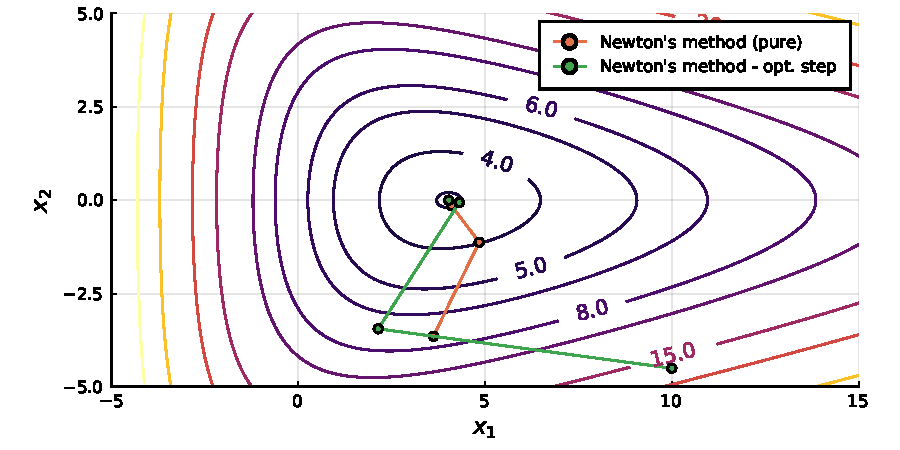
\includegraphics[width=\textwidth]{part_2/chapter_5/figures/newton_path6.pdf}
	\caption{A comparison of the trajectory of both Newton's method variants. Notice that in the method using the exact line search, wile the direction $d = x^* - x_0$ is utilised, the step size is larger in the first iteration.} \label{fig:newton_method_comp}
\end{figure}
%


Algorithm \ref{Alg7} presents a pseudocode for the Newton's method. Notice that in Line \ref{alg7:line3}, an inversion operation is required. One might be cautious about this operation, since as $\nabla f(x_k)$ tends to zero, the Hessian $H(x_k)$ tends to become singular, potentially causing numerical instabilities.

\begin{algorithm}[H]
\caption{Newton's method} \label{Alg7}
\begin{algorithmic}[1] %line numbering frequency. 
\State {\bf initialise.} tolerance $\epsilon > 0,$ initial point $x_0,$ iteration count $k = 0$. 
\While {$||\nabla f(x_k)|| > \epsilon$} 
        \State $d = -H^{-1}(x_k) \nabla f(x_k)$ \label{alg7:line3}
        \State $\overline{\lambda} = \argmin_{\lambda \in \reals}\braces{f(x_k + \lambda d)}$
        \State $x_{k+1} = x_k + \overline{\lambda}  d$
    \State $k = k+1$    
\EndWhile
\State {\bf return} $x_k$
\end{algorithmic}
\end{algorithm}
 
Figure \ref{fig:newton} shows the progression of the Newton's method for $f$ with exact and inexact line searches.

\begin{figure}[H]
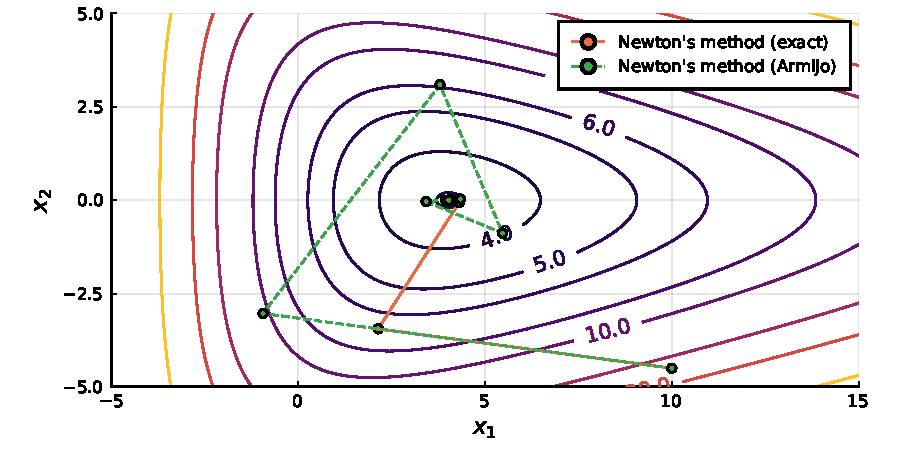
\includegraphics[width=\textwidth]{part_2/chapter_5/figures/newton.pdf}	
\caption{Newton's method applied to $f$. Convergence is observed in 4 steps using exact line search and 27 using Armijo's rule ($\epsilon = 10^{-5}$)} \label{fig:newton}
\end{figure}

